% Options for packages loaded elsewhere
\PassOptionsToPackage{unicode}{hyperref}
\PassOptionsToPackage{hyphens}{url}
\PassOptionsToPackage{dvipsnames,svgnames,x11names}{xcolor}
%
\documentclass[
  12pt,
  letterpaper,
  DIV=11,
  numbers=noendperiod]{scrartcl}

\usepackage{amsmath,amssymb}
\usepackage{iftex}
\ifPDFTeX
  \usepackage[T1]{fontenc}
  \usepackage[utf8]{inputenc}
  \usepackage{textcomp} % provide euro and other symbols
\else % if luatex or xetex
  \usepackage{unicode-math}
  \defaultfontfeatures{Scale=MatchLowercase}
  \defaultfontfeatures[\rmfamily]{Ligatures=TeX,Scale=1}
\fi
\usepackage{lmodern}
\ifPDFTeX\else  
    % xetex/luatex font selection
    \setmainfont[]{Arial}
\fi
% Use upquote if available, for straight quotes in verbatim environments
\IfFileExists{upquote.sty}{\usepackage{upquote}}{}
\IfFileExists{microtype.sty}{% use microtype if available
  \usepackage[]{microtype}
  \UseMicrotypeSet[protrusion]{basicmath} % disable protrusion for tt fonts
}{}
\makeatletter
\@ifundefined{KOMAClassName}{% if non-KOMA class
  \IfFileExists{parskip.sty}{%
    \usepackage{parskip}
  }{% else
    \setlength{\parindent}{0pt}
    \setlength{\parskip}{6pt plus 2pt minus 1pt}}
}{% if KOMA class
  \KOMAoptions{parskip=half}}
\makeatother
\usepackage{xcolor}
\usepackage[a4paper, margin=2.5cm]{geometry}
\setlength{\emergencystretch}{3em} % prevent overfull lines
\setcounter{secnumdepth}{5}
% Make \paragraph and \subparagraph free-standing
\makeatletter
\ifx\paragraph\undefined\else
  \let\oldparagraph\paragraph
  \renewcommand{\paragraph}{
    \@ifstar
      \xxxParagraphStar
      \xxxParagraphNoStar
  }
  \newcommand{\xxxParagraphStar}[1]{\oldparagraph*{#1}\mbox{}}
  \newcommand{\xxxParagraphNoStar}[1]{\oldparagraph{#1}\mbox{}}
\fi
\ifx\subparagraph\undefined\else
  \let\oldsubparagraph\subparagraph
  \renewcommand{\subparagraph}{
    \@ifstar
      \xxxSubParagraphStar
      \xxxSubParagraphNoStar
  }
  \newcommand{\xxxSubParagraphStar}[1]{\oldsubparagraph*{#1}\mbox{}}
  \newcommand{\xxxSubParagraphNoStar}[1]{\oldsubparagraph{#1}\mbox{}}
\fi
\makeatother


\providecommand{\tightlist}{%
  \setlength{\itemsep}{0pt}\setlength{\parskip}{0pt}}\usepackage{longtable,booktabs,array}
\usepackage{calc} % for calculating minipage widths
% Correct order of tables after \paragraph or \subparagraph
\usepackage{etoolbox}
\makeatletter
\patchcmd\longtable{\par}{\if@noskipsec\mbox{}\fi\par}{}{}
\makeatother
% Allow footnotes in longtable head/foot
\IfFileExists{footnotehyper.sty}{\usepackage{footnotehyper}}{\usepackage{footnote}}
\makesavenoteenv{longtable}
\usepackage{graphicx}
\makeatletter
\def\maxwidth{\ifdim\Gin@nat@width>\linewidth\linewidth\else\Gin@nat@width\fi}
\def\maxheight{\ifdim\Gin@nat@height>\textheight\textheight\else\Gin@nat@height\fi}
\makeatother
% Scale images if necessary, so that they will not overflow the page
% margins by default, and it is still possible to overwrite the defaults
% using explicit options in \includegraphics[width, height, ...]{}
\setkeys{Gin}{width=\maxwidth,height=\maxheight,keepaspectratio}
% Set default figure placement to htbp
\makeatletter
\def\fps@figure{htbp}
\makeatother

\KOMAoption{captions}{tableheading}

\makeatletter
\@ifpackageloaded{caption}{}{\usepackage{caption}}
\AtBeginDocument{%
\ifdefined\contentsname
  \renewcommand*\contentsname{Table of contents}
\else
  \newcommand\contentsname{Table of contents}
\fi
\ifdefined\listfigurename
  \renewcommand*\listfigurename{List of Figures}
\else
  \newcommand\listfigurename{List of Figures}
\fi
\ifdefined\listtablename
  \renewcommand*\listtablename{List of Tables}
\else
  \newcommand\listtablename{List of Tables}
\fi
\ifdefined\figurename
  \renewcommand*\figurename{Figure}
\else
  \newcommand\figurename{Figure}
\fi
\ifdefined\tablename
  \renewcommand*\tablename{Table}
\else
  \newcommand\tablename{Table}
\fi
}
\@ifpackageloaded{float}{}{\usepackage{float}}
\floatstyle{ruled}
\@ifundefined{c@chapter}{\newfloat{codelisting}{h}{lop}}{\newfloat{codelisting}{h}{lop}[chapter]}
\floatname{codelisting}{Listing}
\newcommand*\listoflistings{\listof{codelisting}{List of Listings}}
\makeatother
\makeatletter
\makeatother
\makeatletter
\@ifpackageloaded{caption}{}{\usepackage{caption}}
\@ifpackageloaded{subcaption}{}{\usepackage{subcaption}}
\makeatother

\ifLuaTeX
  \usepackage{selnolig}  % disable illegal ligatures
\fi
\usepackage{bookmark}

\IfFileExists{xurl.sty}{\usepackage{xurl}}{} % add URL line breaks if available
\urlstyle{same} % disable monospaced font for URLs
\hypersetup{
  pdftitle={Optimización Bayesiana para busqueda de hiperparámetros},
  colorlinks=true,
  linkcolor={blue},
  filecolor={Maroon},
  citecolor={Blue},
  urlcolor={Blue},
  pdfcreator={LaTeX via pandoc}}


\title{Optimización Bayesiana para busqueda de hiperparámetros}
\author{}
\date{}

\begin{document}
\maketitle

\renewcommand*\contentsname{Índice}
{
\hypersetup{linkcolor=}
\setcounter{tocdepth}{3}
\tableofcontents
}

\newpage

\section{Optimización Bayesiana para búsqueda de
hiperparámetros}\label{optimizaciuxf3n-bayesiana-para-buxfasqueda-de-hiperparuxe1metros}

\subsection{Introducción}\label{introducciuxf3n}

En el ámbito de la ciencia de datos y el aprendizaje automático, la
selección de hiperparámetros es una tarea esencial para garantizar el
desempeño óptimo de los modelos predictivos. Los hiperparámetros, a
diferencia de los parámetros ajustados durante el entrenamiento, son
configuraciones definidas previamente que afectan directamente la
capacidad de generalización de los modelos, es decir, su habilidad para
aprender patrones complejos y evitar problemas como el sobreajuste o el
subajuste.

Técnicas como la búsqueda en cuadrícula (\texttt{GridSearch}) y la
búsqueda aleatoria (\texttt{RandomSearch}) han sido ampliamente
utilizadas para esta tarea. Sin embargo, ambas presentan limitaciones
significativas: son computacionalmente costosas en espacios de búsqueda
grandes y carecen de estrategias para priorizar configuraciones
prometedoras.

La optimización bayesiana ha emergido como una solución eficiente y
efectiva para abordar este tipo de desafíos. Esta técnica, combina
principios probabilísticos y de optimización para modelar iterativamente
el espacio de búsqueda. Al construir un modelo probabilístico del
rendimiento del modelo en función de los hiperparámetros, permite
identificar de manera estratégica configuraciones que optimizan métricas
como la pérdida logarítmica o la precisión.

En este proyecto, exploramos la aplicación de la optimización bayesiana
para la búsqueda de hiperparámetros en modelos de aprendizaje automático
y profundo. A través de herramientas como procesos gaussianos (Gaussian
Processes), estimadores Parzen estructurados en árbol (Tree-structured
Parzen Estimators, TPE), y otras metodologías avanzadas, para evaluar su
eficacia frente a enfoques tradicionales. Además, analizaremos sus
beneficios, desafíos y limitaciones, proporcionando un marco claro para
su implementación en proyectos prácticos.

\subsection{Búsqueda de
Hiperparámetros}\label{buxfasqueda-de-hiperparuxe1metros}

La importancia de un ajuste adecuado de hiperparámetros, ha sido
ampliamente reconocida en la literatura científica, ya que puede mejorar
significativamente el rendimiento y la generalización de los modelos.
Existen diversos enfoques descritos, desde métodos manuales hasta
algoritmos automáticos basados en optimización global.

\textbf{Limitaciones de Enfoques Tradicionales}

\begin{enumerate}
\def\labelenumi{\arabic{enumi}.}
\tightlist
\item
  \textbf{Búsqueda en cuadrícula (\emph{Grid Search}):}
\end{enumerate}

ste enfoque realiza una búsqueda exhaustiva, evaluando todas las
combinaciones posibles dentro de un rango predefinido de
hiperparámetros. Aunque garantiza la exploración completa del espacio,
es ineficiente en términos computacionales, especialmente en espacios de
alta dimensión.

\begin{enumerate}
\def\labelenumi{\arabic{enumi}.}
\setcounter{enumi}{1}
\tightlist
\item
  \textbf{Búsqueda aleatoria (\emph{Random Search}):}
\end{enumerate}

Aquí, los hiperparámetros se seleccionan aleatoriamente dentro de los
límites definidos. Aunque mejora la eficiencia respecto al Grid Search,
carece de una estrategia para priorizar configuraciones prometedoras, lo
que resulta en un rendimiento variable en problemas complejos.

\begin{enumerate}
\def\labelenumi{\arabic{enumi}.}
\setcounter{enumi}{2}
\tightlist
\item
  \textbf{Optimización Bayesiana:}
\end{enumerate}

La optimización bayesiana, aborda estas limitaciones al construir un
modelo probabilístico del rendimiento del modelo, en función de los
hiperparámetros. Este enfoque, guía la búsqueda hacia configuraciones
óptimas mediante un equilibrio entre \textbf{exploración} (\emph{probar
regiones poco exploradas}) y \textbf{explotación} (\emph{ajustar
configuraciones prometedoras}).

\begin{figure}[H]

{\centering 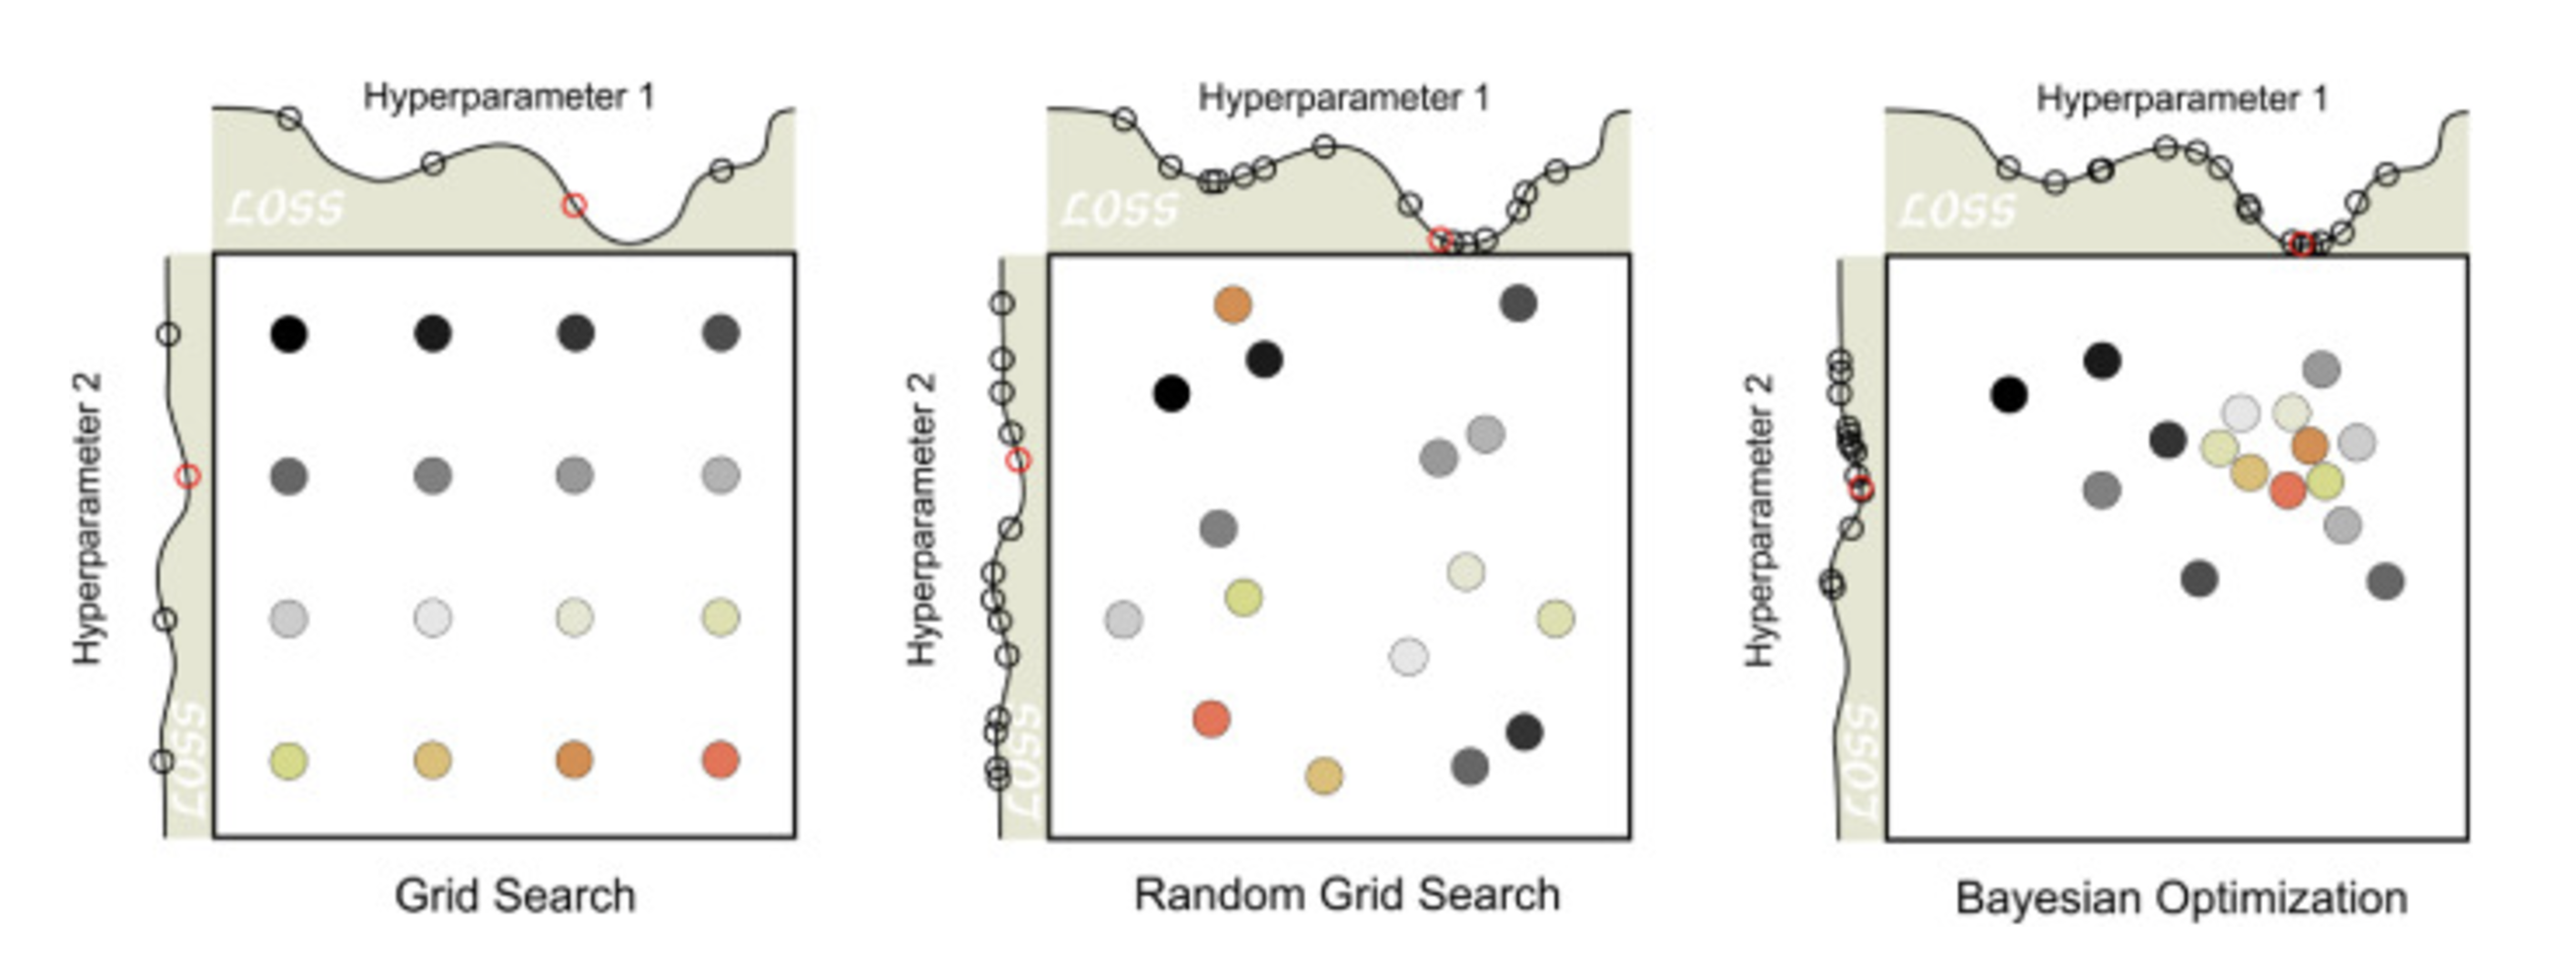
\includegraphics{imgs/Comparacion_Search.png}

}

\caption{Comparativo de enfoques para búsqueda de hiperpárametros}

\end{figure}%

\textbf{Estudios destacados incluyen:}

\begin{itemize}
\tightlist
\item
  En {[}1{]}, se demostró que la optimización bayesiana, aplicada a
  modelos como bosques aleatorios y redes neuronales profundas (CNN,
  RNN), supera en eficiencia y precisión a los enfoques tradicionales.
\item
  En {[}2{]}, se destacó la capacidad del estimador TPE para ajustar
  hasta 32 hiperparámetros en modelos complejos como redes de creencias
  profundas (DBN).
\item
  En {[}3{]}, se validó la superioridad de la optimización bayesiana en
  términos de velocidad y rendimiento, especialmente en espacios de
  búsqueda de alta dimensión o recursos computacionales limitados.
\end{itemize}

\subsection{Optimización de
Hiperparámetros}\label{optimizaciuxf3n-de-hiperparuxe1metros}

El ajuste de hiperparámetros puede entenderse como un problema de
optimización de funciones de caja negra (\emph{BlackBox}), donde la
función objetivo (por ejemplo, la métrica de evaluación del modelo) no
tiene una expresión cerrada, ni derivadas accesibles. Esto dificulta el
uso de métodos tradicionales como el descenso de gradiente.

\subsubsection{Enfoques Automáticos}\label{enfoques-automuxe1ticos}

\begin{enumerate}
\def\labelenumi{\arabic{enumi}.}
\tightlist
\item
  \textbf{Grid Search}:
\end{enumerate}

Proporciona un marco exhaustivo, pero enfrenta la maldición de la
dimensionalidad, limitando su aplicabilidad en problemas complejos.

\begin{enumerate}
\def\labelenumi{\arabic{enumi}.}
\setcounter{enumi}{1}
\tightlist
\item
  \textbf{Random Search}:
\end{enumerate}

Aunque más eficiente, carece de una estrategia para explotar información
previa o configuraciones prometedoras.

\subsubsection{Ventajas de la Optimización
Bayesiana}\label{ventajas-de-la-optimizaciuxf3n-bayesiana}

Integra información previa sobre el espacio de búsqueda, para actualizar
la distribución posterior iterativamente. Utiliza funciones de
adquisición, para decidir las siguientes configuraciones a probar,
optimizando recursos computacionales.Es decir, modela el rendimiento del
modelo de manera probabilística, permitiendo una exploración más
eficiente y efectiva del espacio de hiperparámetros.

\begin{figure}[H]

{\centering 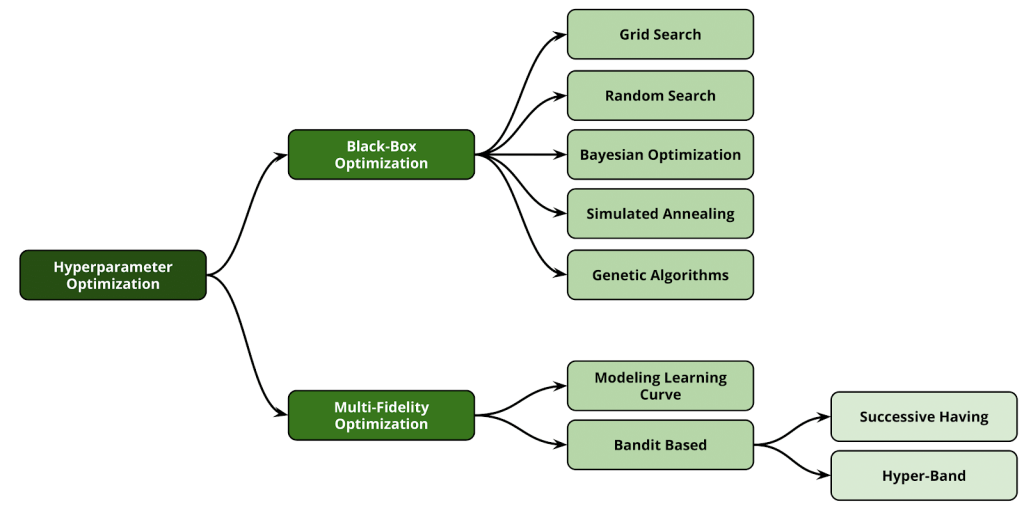
\includegraphics{imgs/esquema_enfoques_HPO.png}

}

\caption{Esquema de enfoques en la búsqueda de hiperpárametros}

\end{figure}%

\subsection{Fundamentos Matemáticos de la Optimización
Bayesiana}\label{fundamentos-matemuxe1ticos-de-la-optimizaciuxf3n-bayesiana}

La optimización bayesiana busca maximizar una función objetivo \(f(x)\)
desconocida en un espacio de búsqueda \(A\), utilizando el siguiente
enfoque:

\[
x^+ = \underset{x \in A}{\text{arg max }} f(x) : \tag{1}
\]

Se basa en el \href{https://arxiv.org/pdf/1012.2599.pdf}{teorema de
Bayes}, el cual establece que, dado un conjunto de datos evidenciales
\(E\), la probabilidad posterior \(P(M|E)\) de un modelo \(M\), es
proporcional a la probabilidad \(P(E|M)\), de observar \(E\), dado el
modelo \(M\), multiplicada por la probabilidad previa \(P(M)\):

\[
P(M|E) \propto P(E|M)P(M) : \tag{2}
\]

La fórmula anterior, refleja la idea central de la optimización
bayesiana. El principio consiste en combinar la distribución previa de
la función \(f(x)\) con la información de las muestras (evidencia) para
obtener la distribución posterior de la función. Luego, se utiliza esta
información posterior para determinar dónde se maximiza la función
\(f(x)\) según un criterio. En otras palabras,combina una distribución
previa, con evidencia obtenida durante la búsqueda, para actualizar la
distribución posterior de \(f(x)\).

El criterio se representa mediante una función de utilidad \(u\),
también llamada \textbf{función de adquisición}. La función \(u\) se
utiliza para determinar el siguiente punto de muestreo, con el fin de
maximizar la utilidad esperada. Al explorar el área de muestreo, es
necesario considerar tanto la exploración (muestreo en áreas de alta
incertidumbre), como la explotación (muestreo en áreas con valores
altos). Este equilibrio ayuda a reducir el número de muestras necesarias
y mejora el rendimiento, incluso cuando la función tiene múltiples
máximos locales.

\subsubsection{Proceso Gaussiano (GP)}\label{proceso-gaussiano-gp}

Es una técnica, basada en la teoría de probabilidad gaussiana y
aprendizaje bayesiano. A diferencia de una distribución gaussiana, que
describe variables escalares o vectores, un proceso gaussiano describe
\textbf{propiedades de funciones}. Específicamente, un proceso
gaussiano, asume que cualquier subconjunto finito de valores aleatorios
sigue una distribución gaussiana multivariada.

Un GP se define por su función media \(m(x)\) y su función de covarianza
\(k(x, x')\), representado como:

\[
f(x) \sim GP(m(x), k(x, x'))
\]

\begin{itemize}
\tightlist
\item
  \textbf{Función de Covarianza}
\end{itemize}

Una función común para \(k(x_i, x_j)\), es la exponencial cuadrada:

\[
k(x_i, x_j) = \exp\left(-\frac{1}{2} \|x_i - x_j\|^2\right)
\] donde \(x_i\) y \(x_j\) son puntos de muestreo. Si \(x_i\) y \(x_j\)
están cerca, \(k(x_i, x_j)\) se aproxima a 1; de lo contrario, tiende a
0. Esto representa la correlación y la influencia mutua entre los
puntos.

\begin{itemize}
\tightlist
\item
  \textbf{Predicción y Varianza:}
\end{itemize}

Se calcula la media \(\mu_{t+1}(x_{t+1})\) y varianza
\(\sigma^2_{t+1}(x_{t+1})\) para determinar el siguiente punto a
evaluar.

\begin{figure}[H]

{\centering 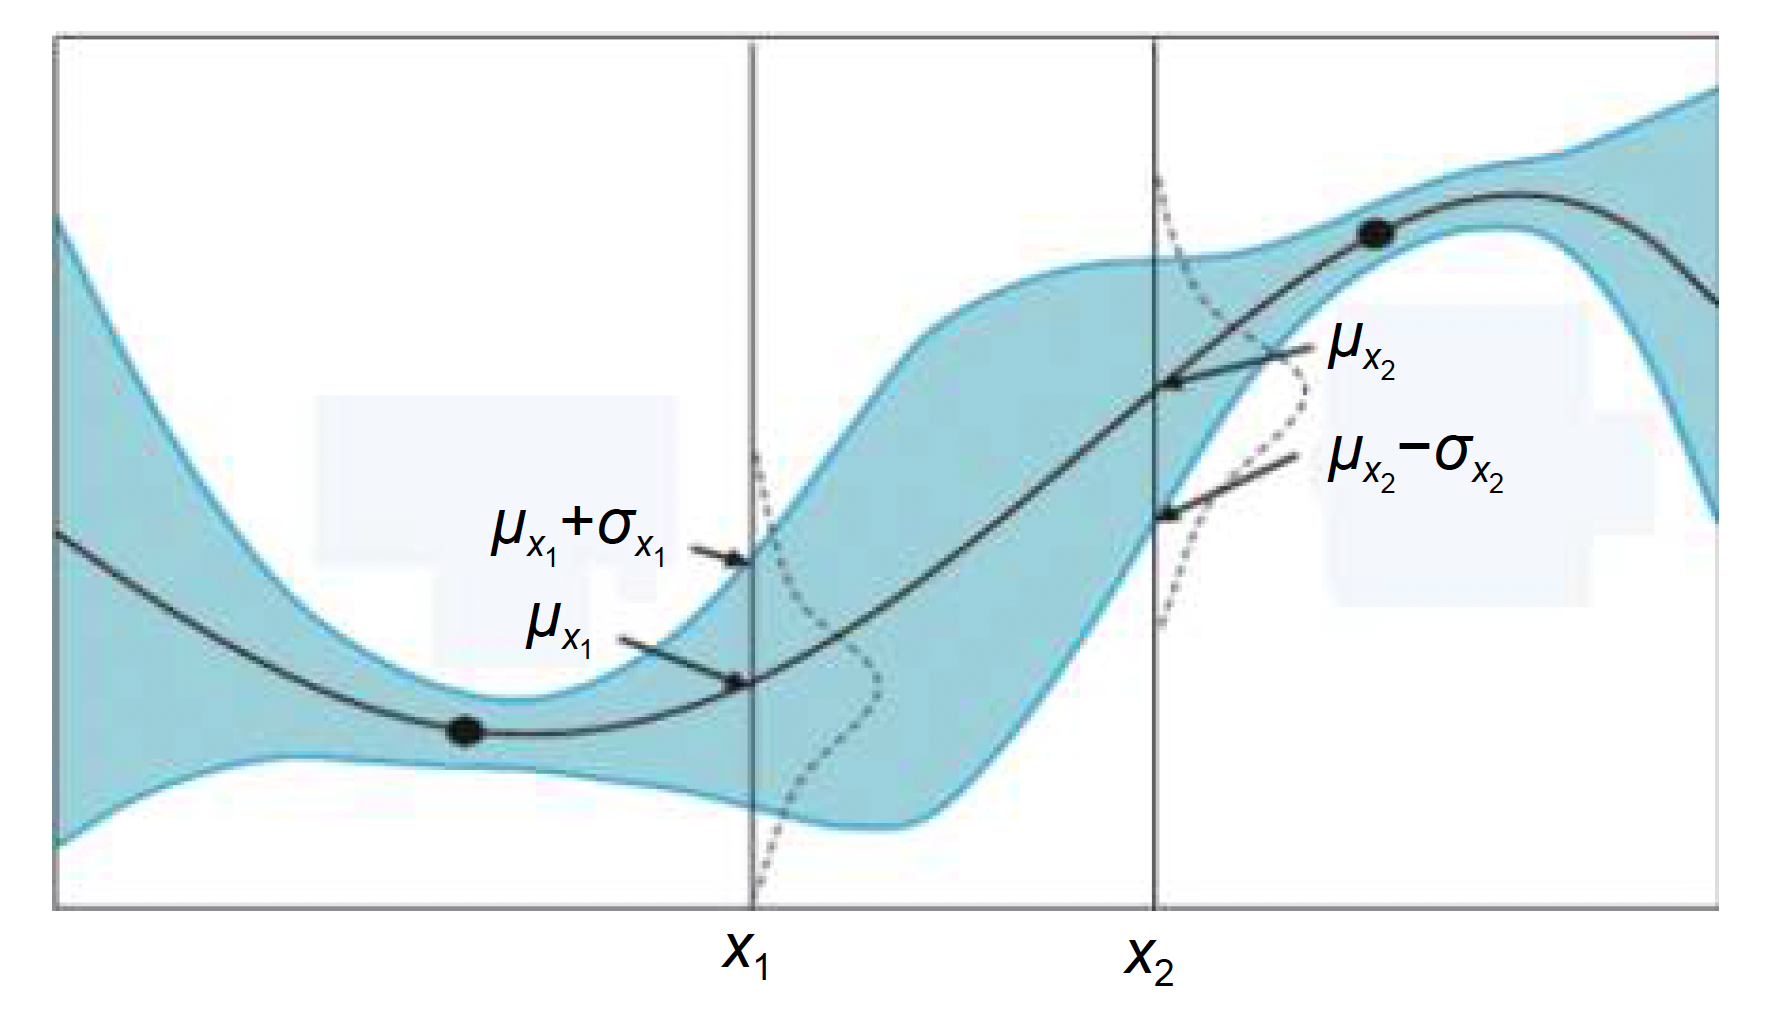
\includegraphics{imgs/Proceso_Gaussiano_1Dim.png}

}

\caption{Fuente (3) Proceso Gaussiano}

\end{figure}%

\subsubsection{Función de
Adquisición}\label{funciuxf3n-de-adquisiciuxf3n}

La función de adquisición o función de utilidad \(u(x)\), determina el
próximo punto a muestrear, equilibrando exploración y explotación con el
fin de maximizar la utilidad esperada. Al explorar el área de muestreo,
es necesario considerar tanto la exploración (muestreo en áreas de alta
incertidumbre), como la explotación (muestreo en áreas con valores
altos). Este equilibrio ayuda a reducir el número de muestras necesarias
y mejora el rendimiento, incluso cuando la función tiene múltiples
máximos locales. Ejemplos:

\begin{enumerate}
\def\labelenumi{\arabic{enumi}.}
\tightlist
\item
  \textbf{Probabilidad de Mejora (PI)}
\end{enumerate}

La función PI, busca puntos donde el valor de \(f(x)\) sea mayor al
valor óptimo actual \(f(x^+)\). La probabilidad de mejora se expresa
como: \[
PI(x) = P(f(x) \geq f(x^+)) = \Phi\left(\frac{\mu(x) - f(x^+)}{\sigma(x)}\right),
\] donde \(\Phi(\cdot)\) es la función de distribución acumulativa de la
normal estándar. Una versión extendida de PI introduce un parámetro
\(\epsilon\) para garantizar que el nuevo punto muestreado supere al
óptimo actual por al menos \(\epsilon\): \[
PI(x) = \Phi\left(\frac{\mu(x) - f(x^+) - \epsilon}{\sigma(x)}\right).
\]

\begin{enumerate}
\def\labelenumi{\arabic{enumi}.}
\setcounter{enumi}{1}
\tightlist
\item
  \textbf{Mejora Esperada (EI)}
\end{enumerate}

La función EI, calcula la expectativa del grado de mejora que puede
lograrse al explorar un punto cerca del óptimo actual. La mejora
esperada se define como: \[
I(x) = \max\{0, f_{t+1}(x) - f(x^+)\}.
\] Maximizamos la EI respecto al valor óptimo actual \(f(x^+)\): \[
x = \underset{x}{\text{arg max }} E[I(x)].
\] La expresión para EI es: \[
E(I) = \sigma(x) \left[ Z \Phi(Z) + \phi(Z) \right],
\] donde

\(Z = \frac{\mu(x) - f(x^+)}{\sigma(x)}\), \(\Phi(\cdot)\) es la función
acumulativa y

\(\phi(\cdot)\) es la densidad de probabilidad de la normal estándar.

\begin{enumerate}
\def\labelenumi{\arabic{enumi}.}
\setcounter{enumi}{2}
\tightlist
\item
  \textbf{Límite Superior de Confianza (GP-UCB)}
\end{enumerate}

La función GP-UCB, decide si el próximo punto a muestrear debe explotar
el valor óptimo actual (zona de alta \(\mu(x)\)) o explorar zonas de
alta incertidumbre \((\sigma(x))\). El equilibrio se controla mediante
el parámetro \(\kappa\): \[
UCB(x) = \mu(x) + \kappa \sigma(x).
\]

En la siguiente imagen se compara el rendimiento de las funciones PI, EI
y GP-UCB en el proceso de optimización. Las líneas azules representan la
media posterior, mientras que las áreas sombreadas muestran la
incertidumbre (\(\pm \sigma(x)\)). EI y GP-UCB logran encontrar el valor
global óptimo, mientras que PI tiende a quedarse atrapada en óptimos
locales debido a su naturaleza codiciosa.

\begin{figure}[H]

{\centering 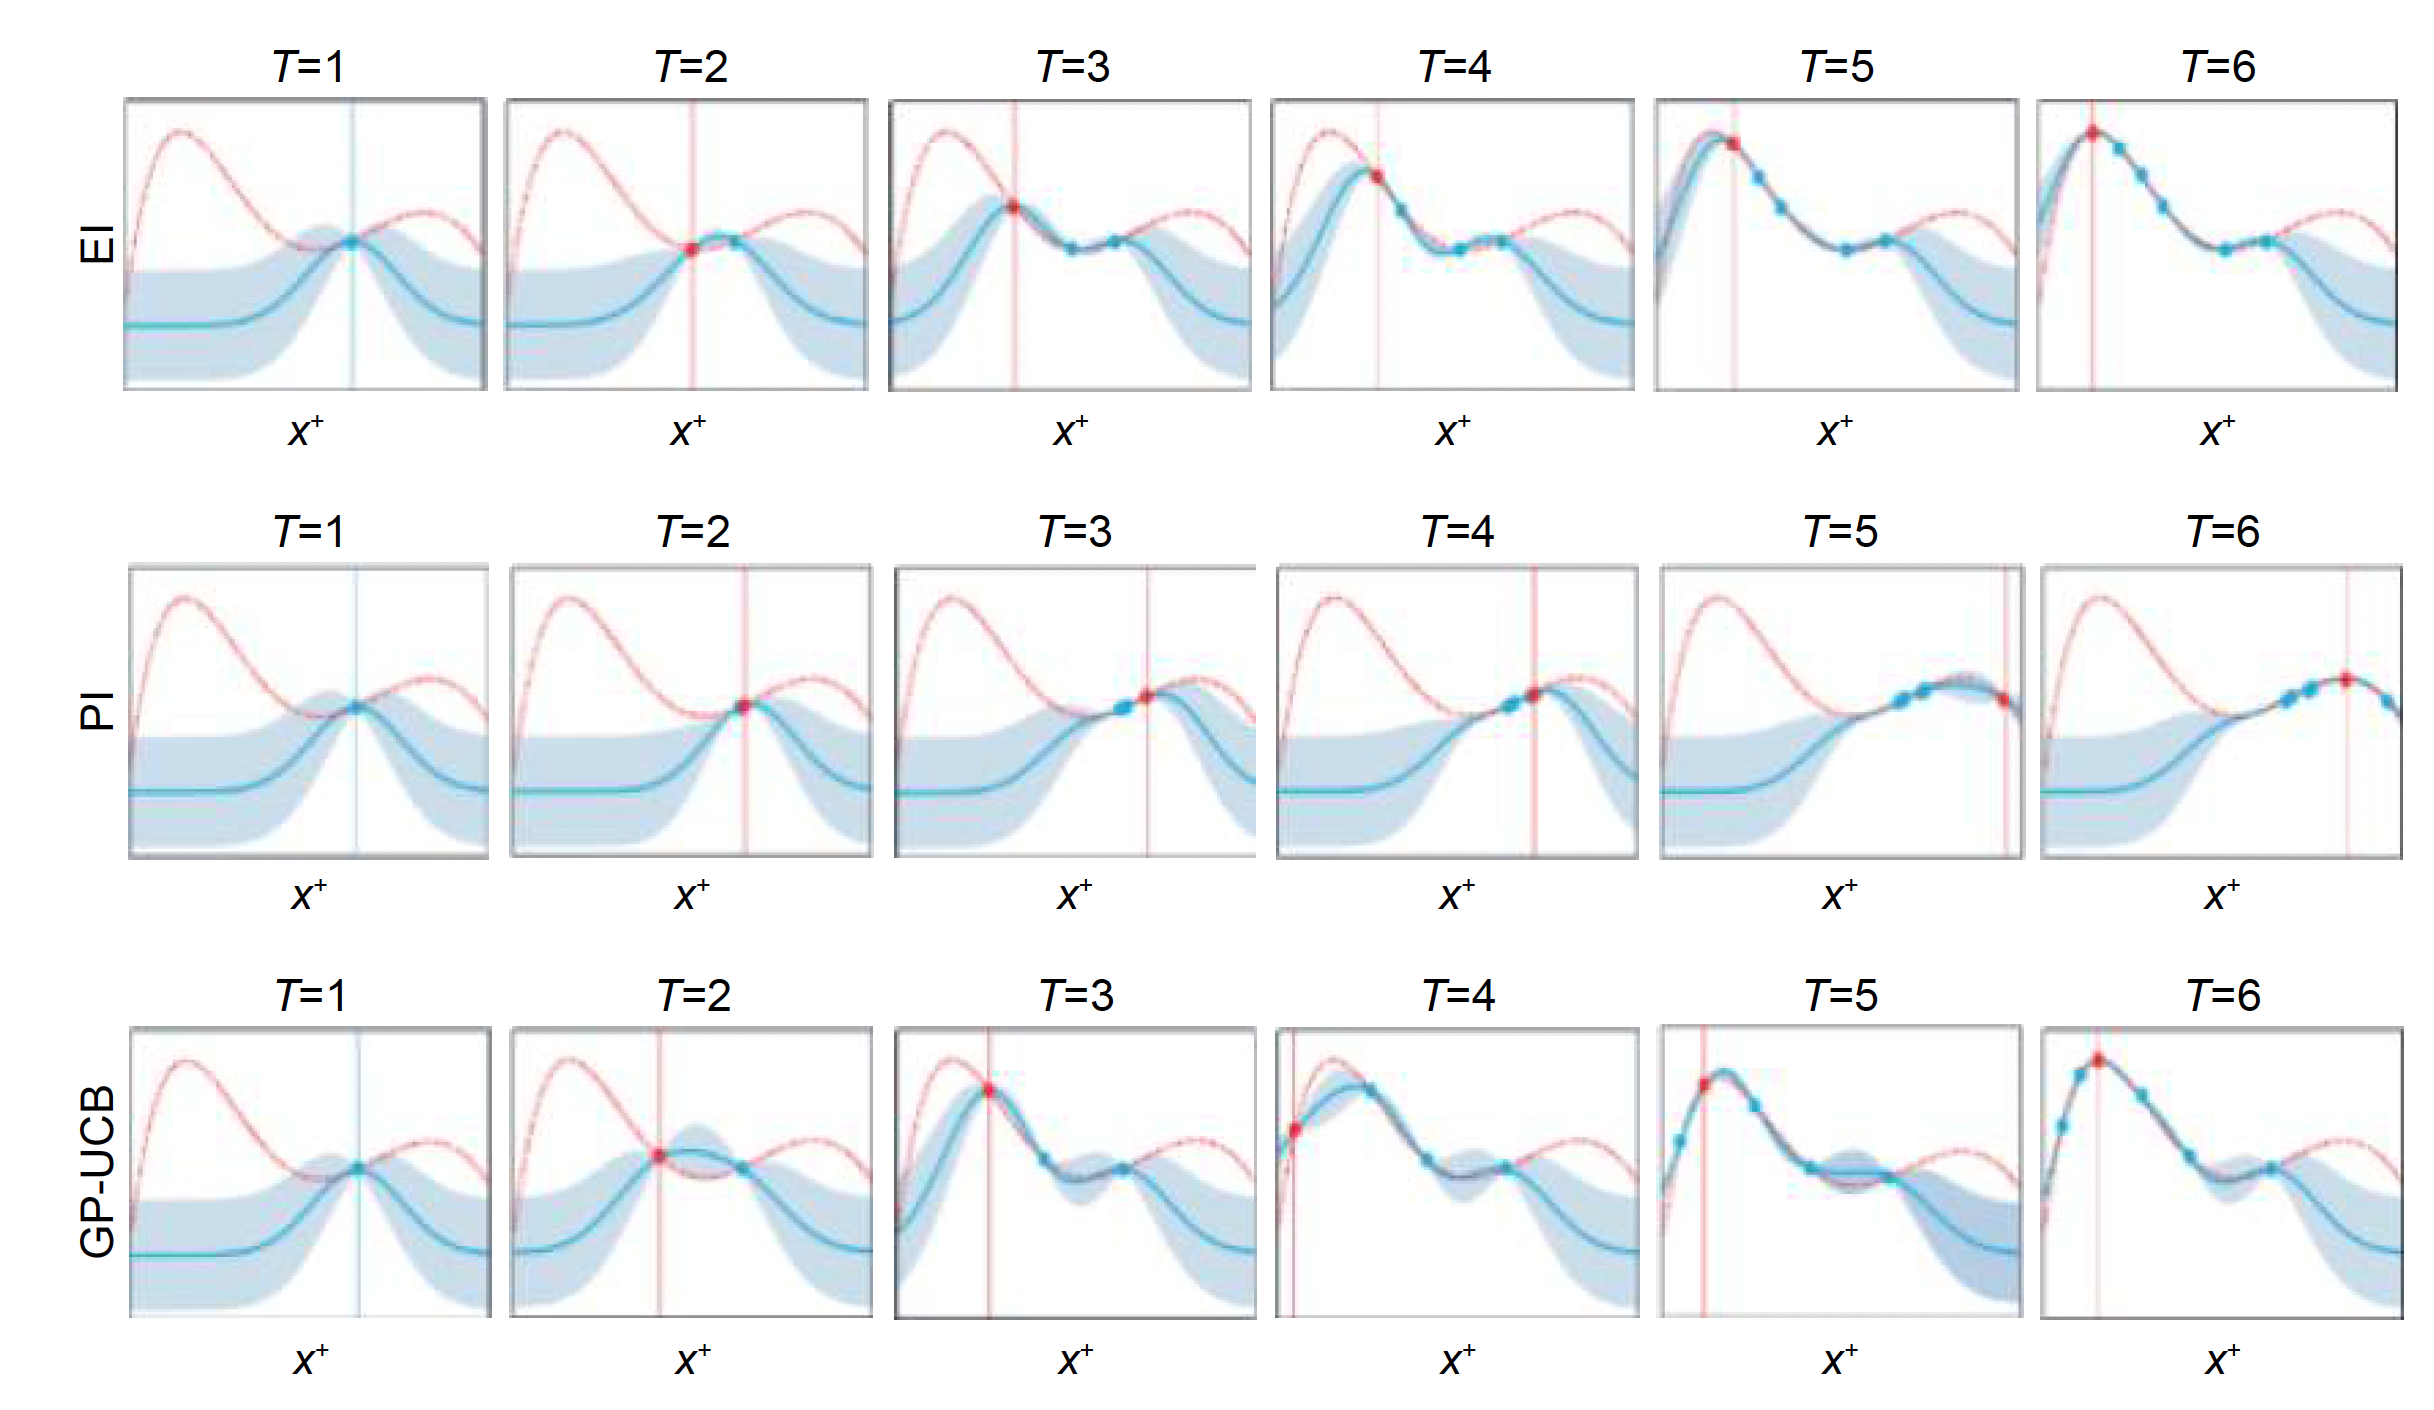
\includegraphics{imgs/image.png}

}

\caption{Fuente (3) Comparación de funciones de adquisición)}

\end{figure}%

Según los resultados experimentales, la función EI es ideal para
optimizar hiperparámetros por su simplicidad y rendimiento superior en
comparación con PI y GP-UCB. Sin embargo, la elección de la función de
adquisición depende del problema y la función objetivo, por lo que es
recomendable probar varias funciones para determinar la más adecuada.

\subsection{Implementación con NumPy y
SciPy}\label{implementaciuxf3n-con-numpy-y-scipy}

En esta sección, implementaremos la función de adquisición y su
optimización en NumPy y SciPy, así mismo usaremos scikit-learn para la
el proceso gaussiano. Aunque tenemos una expresión analítica del
objetivo de optimización \texttt{f} en el siguiente ejemplo, lo tratamos
como una \texttt{Black-Box} y lo aproximamos iterativamente con un
proceso gaussiano durante la optimización bayesiana. Además, las
muestras extraídas de la función objetivo son ruidosas y el nivel de
ruido está dado por la variable \texttt{noise}. La optimización se
realiza dentro de los \texttt{límites} dados. También asumimos que
existen dos muestras iniciales en \texttt{X\_init} e \texttt{Y\_init}.

Función: \[
f(X)=-\sin(3X)-X^2+0.7X + \text{noise}*\text{randn}
\]

La siguiente gráfica muestra: - La función objetivo libre de ruido - La
cantidad de ruido al representar gráficamente una gran cantidad de
muestras y - Las dos muestras iniciales

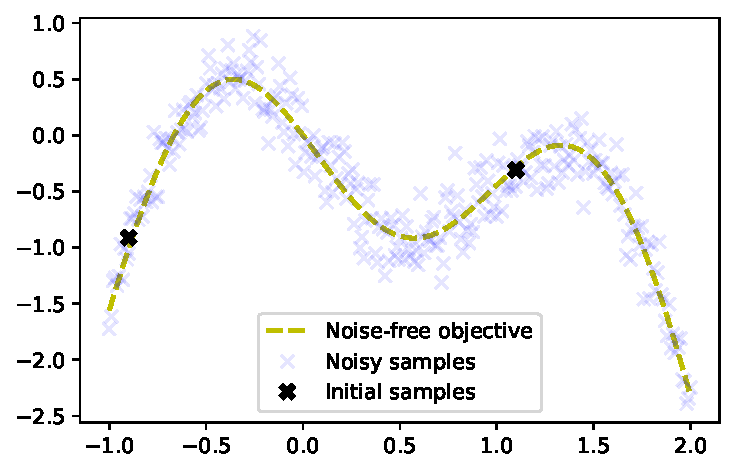
\includegraphics{ProyFinal_OptBayesiana_2024_files/figure-pdf/cell-3-output-1.pdf}

El objetivo, \textbf{es encontrar el óptimo global a la izquierda}, en
una pequeña cantidad de pasos. El siguiente paso es implementar la
función de adquisición definida como función EI
(\texttt{expected\_improvement}).

También necesitamos una función que proponga el siguiente punto de
muestreo, calculando la ubicación del máximo de la función de
adquisición. La optimización se reinicia \texttt{n\_restarts} veces para
evitar óptimos locales.

Ahora tenemos todos los componentes necesarios para ejecutar la
optimización bayesiana con el algoritmo descrito anteriormente. El
proceso gaussiano del siguiente ejemplo está configurado con un
\href{http://scikit-learn.org/stable/modules/gaussian_process.html\#matern-kernel}{Matérn
kernel}. El nivel de ruido conocido se configura con el parámetro
\texttt{alpha}.

La optimización bayesiana, se ejecuta durante 10 iteraciones. En cada
iteración, produce una fila con dos gráficos.

\begin{itemize}
\tightlist
\item
  El gráfico de la izquierda muestra la función objetivo sin ruido,
  \textbf{la función sustituta}, que es la media predictiva posterior de
  Gaussian Process, el intervalo de confianza es de 95\% de la media y
  las muestras ruidosas obtenidas de la función objetivo hasta el
  momento.
\item
  El gráfico de la derecha muestra la función de adquisición.
\item
  La línea discontinua vertical en ambos gráficos muestra el punto de
  muestreo propuesto para la siguiente iteración, que corresponde al
  máximo de la función de adquisición.
\end{itemize}

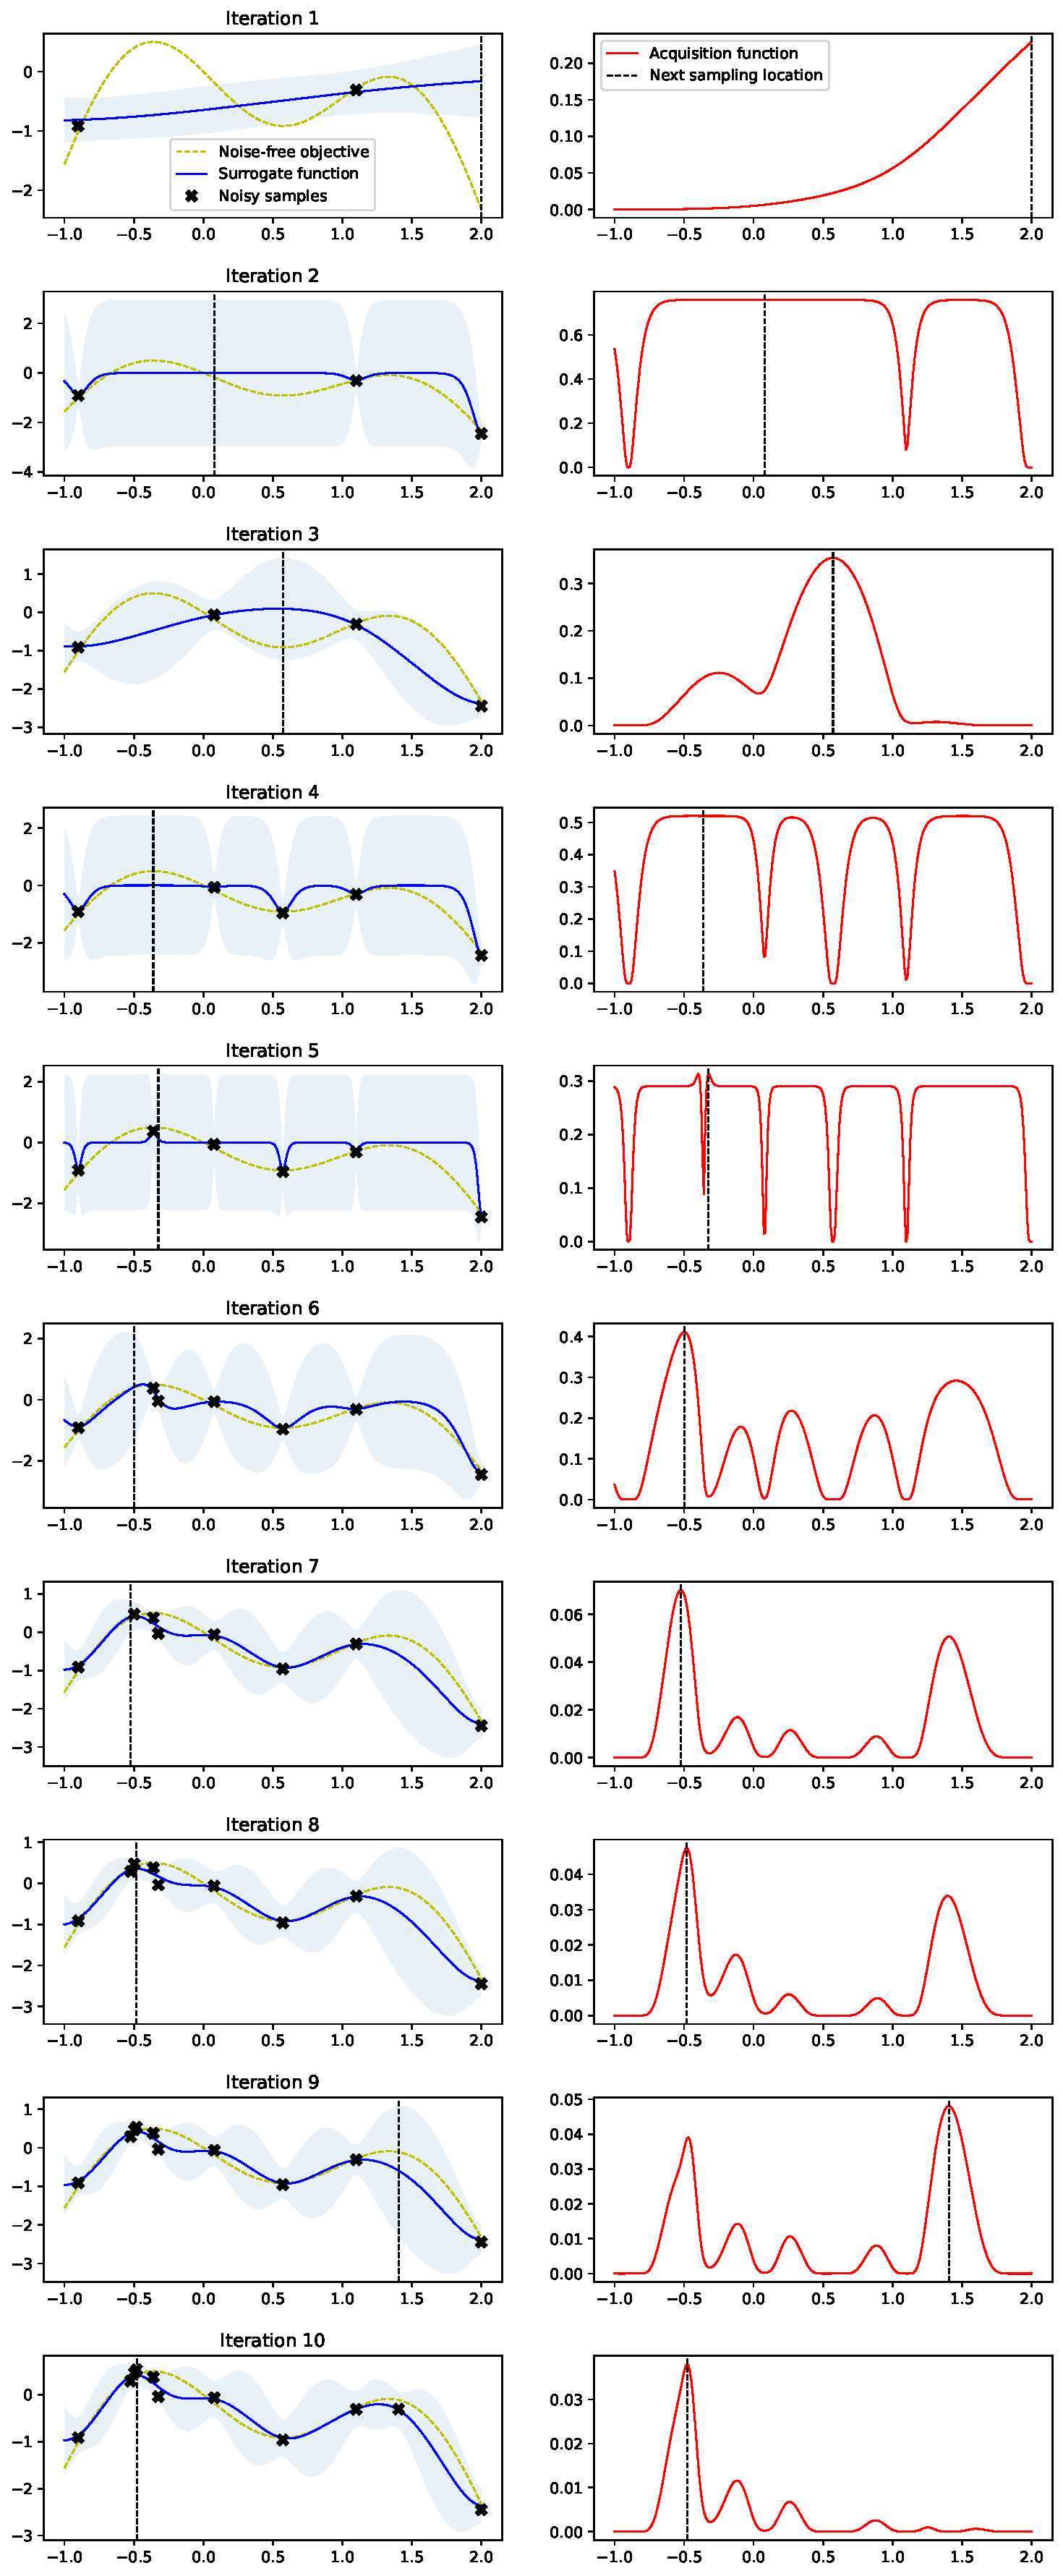
\includegraphics{ProyFinal_OptBayesiana_2024_files/figure-pdf/cell-6-output-1.pdf}

Se puede observar, cómo las dos muestras iniciales dirigen la búsqueda
hacia la dirección del máximo local en el lado derecho, pero la
exploración, permite que el algoritmo escape de ese óptimo local y
encuentre el óptimo global en el lado izquierdo.

Así mismo se observa también cómo las propuestas de puntos de muestreo,
a menudo caen dentro de regiones de alta incertidumbre (exploración) y
no solo están impulsadas por los valores más altos de la función
sustituta (explotación).

Un gráfico de convergencia revela cuántas iteraciones se necesitan para
encontrar un máximo y si las propuestas de puntos de muestreo se
mantienen alrededor de ese máximo, es decir, convergen a pequeñas
diferencias entre pasos consecutivos.

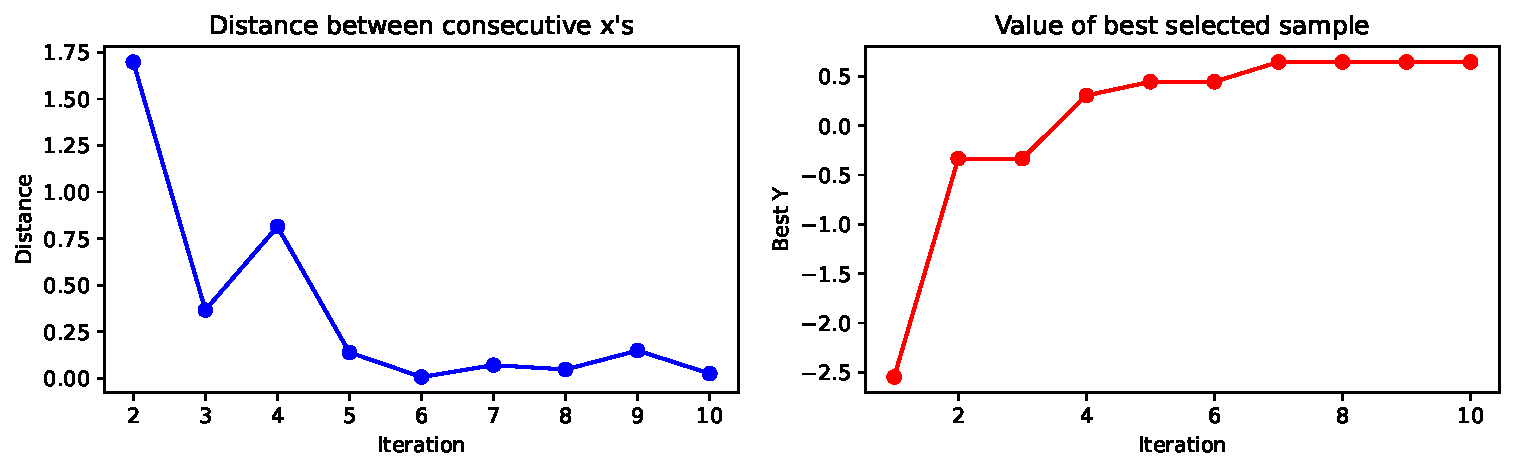
\includegraphics{ProyFinal_OptBayesiana_2024_files/figure-pdf/cell-7-output-1.pdf}

\subsection{Librerias para la Optimización
Bayesiana}\label{librerias-para-la-optimizaciuxf3n-bayesiana}

Existen numerosas librerias de optimización bayesiana y el objetivo de
este análisis no es brindar una descripción general de estas, sino, de
ejemplificar dos y mostrar la configuración mínima necesaria para
ejecutar el ejemplo anterior.

\subsubsection{Scikit-Optimize}\label{scikit-optimize}

\href{https://scikit-optimize.github.io/}{Scikit-optimize} es una
biblioteca para la optimización basada en modelos secuenciales que se
basa en \href{https://numpy.org/}{NumPy},
\href{https://scipy.org/}{SciPy} y
\href{http://scikit-learn.org/}{Scikit-Learn}. También admite la
optimización bayesiana mediante procesos gaussianos. La API está
diseñada entorno a la minimización, por lo tanto, tenemos que
proporcionar valores de función objetivo negativos. Los resultados
obtenidos aquí difieren ligeramente de los resultados anteriores debido
al comportamiento de optimización no determinista y a las diferentes
muestras ruidosas extraídas de la función objetivo.

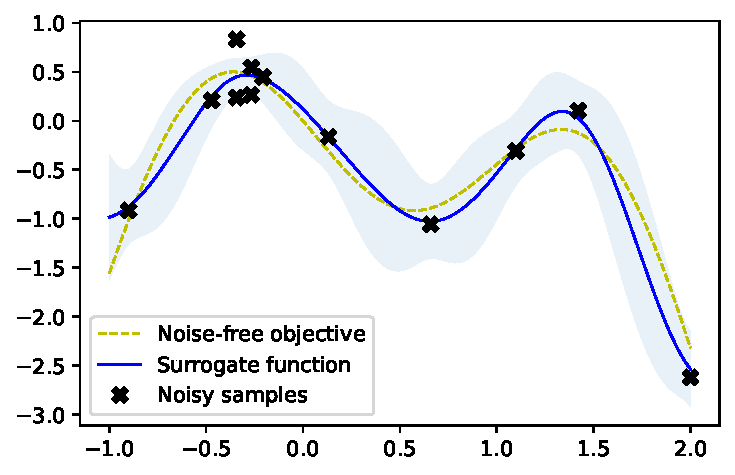
\includegraphics{ProyFinal_OptBayesiana_2024_files/figure-pdf/cell-8-output-1.pdf}

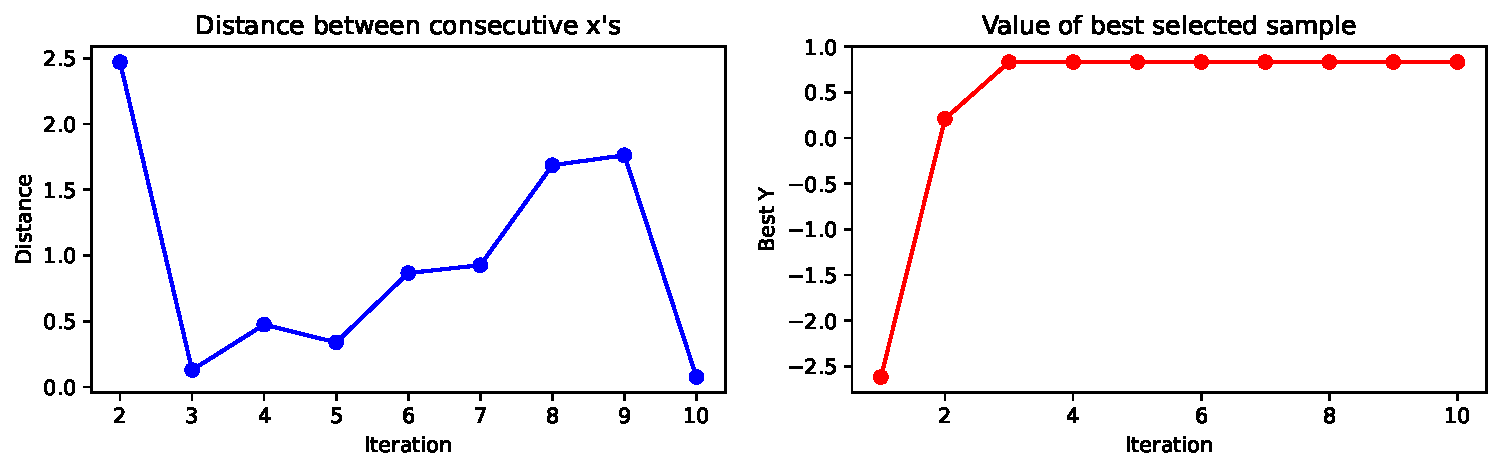
\includegraphics{ProyFinal_OptBayesiana_2024_files/figure-pdf/cell-9-output-1.pdf}

\subsubsection{GPyOpt}\label{gpyopt}

\href{http://sheffieldml.github.io/GPyOpt/}{GPyOpt} es una biblioteca de
optimización bayesiana basada en
\href{https://sheffieldml.github.io/GPy/}{GPy}. El nivel de abstracción
de la API, es comparable al de scikit-optimize. La API
\texttt{BayesianOptimization} proporciona un parámetro \texttt{maximize}
para configurar si la función objetivo se maximizará o minimizará
(predeterminado). En la versión 1.2.1, esto parece ignorarse al
proporcionar muestras iniciales, por lo que tenemos que negar sus
valores objetivo manualmente en el siguiente ejemplo. Además, los
métodos integrados \texttt{plot\_acquisition} y
\texttt{plot\_convergence} muestran el resultado de la minimización en
cualquier caso. Nuevamente, los resultados obtenidos aquí difieren
ligeramente de los resultados anteriores debido al comportamiento de
optimización no determinista y a las diferentes muestras ruidosas
extraídas de la función objetivo.

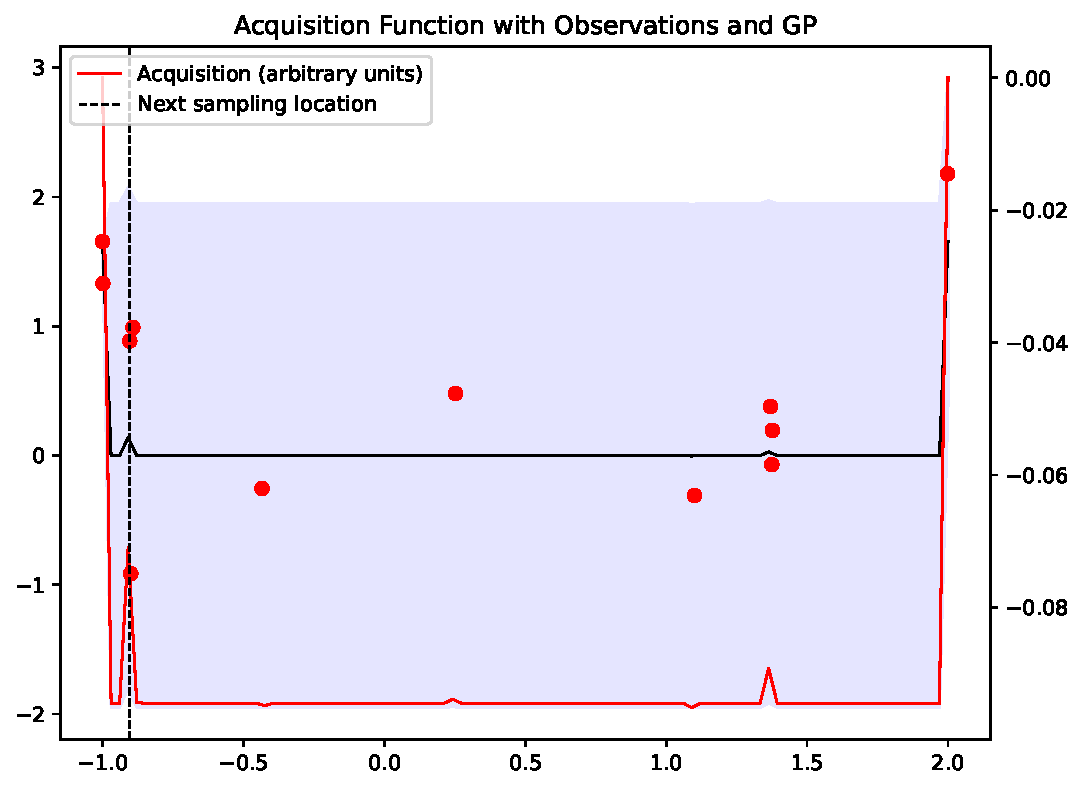
\includegraphics{ProyFinal_OptBayesiana_2024_files/figure-pdf/cell-10-output-1.pdf}

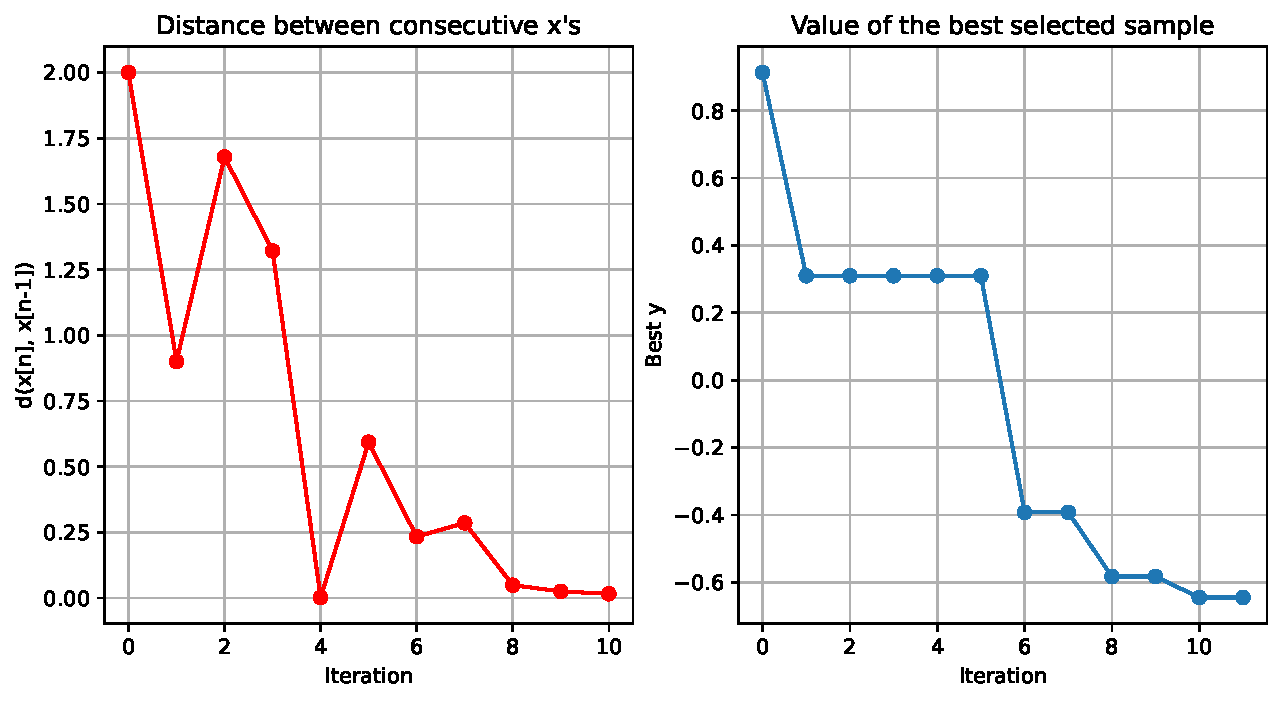
\includegraphics{ProyFinal_OptBayesiana_2024_files/figure-pdf/cell-11-output-1.pdf}

\subsection{Aplicación de Optimización Bayesiana en Aprendizaje
Automático}\label{aplicaciuxf3n-de-optimizaciuxf3n-bayesiana-en-aprendizaje-automuxe1tico}

\subsubsection{Diabetes}\label{diabetes}

En esta sección, aplicaremos la optimización bayesiana a un problema de
regresión. La regresión se realiza en un pequeño
\href{http://scikit-learn.org/stable/modules/generated/sklearn.datasets.load_diabetes.html\#sklearn.datasets.load_diabetes}{conjunto
de datos sobre diabetes} que es parte de scikit-learn.

El conjunto de datos, contiene 10 variables basales como son: edad,
sexo, índice de masa corporal, presión arterial media y 6 mediciones de
suero sanguíneo para cada uno de los 442 pacientes diabéticos, así como
la respuesta del paciente, una medida cuantitativa de la progresión de
la enfermedad, un año después de la toma inicial.

\begin{longtable}[]{@{}
  >{\raggedright\arraybackslash}p{(\columnwidth - 2\tabcolsep) * \real{0.4211}}
  >{\raggedright\arraybackslash}p{(\columnwidth - 2\tabcolsep) * \real{0.5789}}@{}}
\toprule\noalign{}
\begin{minipage}[b]{\linewidth}\raggedright
Atributo
\end{minipage} & \begin{minipage}[b]{\linewidth}\raggedright
Descripción
\end{minipage} \\
\midrule\noalign{}
\endhead
\bottomrule\noalign{}
\endlastfoot
age & age in years \\
sex & sex \\
bmi & body mass index \\
bp & average blood pressure \\
s1 tc & total serum cholesterol \\
s2 ldl & low-density lipoproteins \\
s3 hdl & high-density lipoproteins \\
s4 tch & total cholesterol / HDL \\
s5 ltg & possibly log of serum triglycerides level \\
s6 glu & blood sugar level \\
y & quantitative measure of disease progression one year after
baseline \\
\end{longtable}

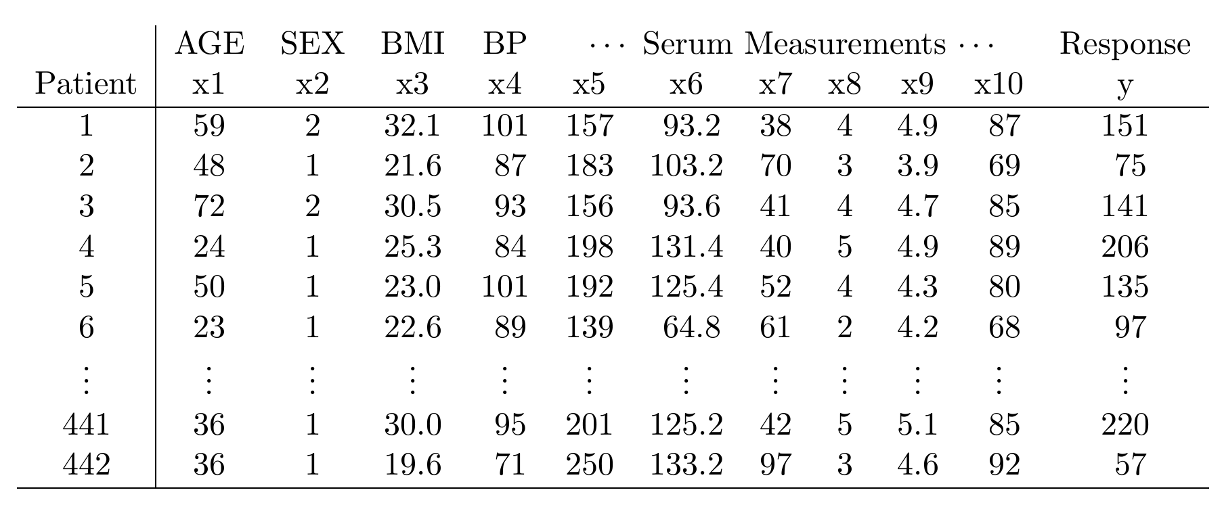
\includegraphics{imgs/data_diabetes.png} Fuente
\href{https://web.stanford.edu/~hastie/Papers/LARS/LeastAngle_2002.pdf}{Diabetes
Study}

\textbf{1. Definición del problema} El objetivo, es predecir la
progresión de la enfermedad un año después del estudio, basándose en
múltiples características explicativas proporcionadas en el conjunto de
datos, utilizando un \texttt{XGBRegressor} con optimización bayesiana
para la búsqueda de hiperparámetros. En esta sección demostraremos cómo
optimizar los hiperparámetros de un \texttt{XGBRegressor} con GPyOpt y
skopt y cómo se compara el rendimiento de la optimización bayesiana
\texttt{BayesianOptimization} con la búsqueda aleatoria
\texttt{RandomSearch}.

Matemáticamente, esto se modela como:

\[
Y = f(X; \Theta) + \epsilon
\]

Donde: - \(Y \in \mathbb{R}\) representa la variable objetivo (medida de
progreso de la enfermedad). - \(X \in \mathbb{R}^{n \times d}\) es la
matriz de entrada con \(n\) muestras y \(d\) características. -
\(\Theta\) representa los hiperparámetros del modelo que afectan su
capacidad de generalización. - \(\epsilon\) es un término de error
(ruido) que modela incertidumbre o variabilidad no explicada por
\(f(X; \Theta)\).

El modelo objetivo \(f(X; \Theta)\) es un \texttt{XGBRegressor} (modelo
de boosting basado en árboles) que tiene múltiples hiperparámetros a
optimizar.

\textbf{2. Función objetivo para la optimización}

El problema de ajuste de hiperparámetros se puede expresar como un
problema de minimización, donde se busca el conjunto de hiperparámetros
\(\Theta^*\) que minimice el error cuadrático medio (MSE) en validación
cruzada:

\[
\Theta^* = \underset{\Theta}{\text{argmin}} \, \frac{1}{k} \sum_{i=1}^{k} \left( \frac{1}{n_i} \sum_{j=1}^{n_i} \left( y_{ij} - \hat{y}_{ij}(\Theta) \right)^2 \right)
\]

Donde: - \(k\) es el número de pliegues en la validación cruzada. -
\(n_i\) es el número de muestras en el pliegue \(i\). - \(y_{ij}\) es el
valor real de la muestra \(j\) en el pliegue \(i\). -
\(\hat{y}_{ij}(\Theta)\) es la predicción realizada por el modelo con
hiperparámetros \(\Theta\).

\textbf{3. Hiperparámetros optimizados}

Los hiperparámetros ajustados (\(\Theta\)) incluyen: 1. \textbf{Tasa de
aprendizaje (\(\eta\))}: Controla la contribución de cada árbol en el
modelo final. - Rango: \([0.01, 1.0]\) 2. \textbf{Profundidad máxima de
los árboles (\(d\))}: Controla la complejidad de los árboles. - Rango:
\([1, 50]\) 3. \textbf{Número de estimadores (\(n_{\text{trees}}\))}:
Número total de árboles en el modelo. - Rango: \([1, 300]\) 4.
\textbf{Peso mínimo de las hojas (\(w_{\text{min}}\))}: Peso mínimo
requerido para dividir un nodo. - Rango: \([1, 10]\) 5.
\textbf{Parámetro \(\gamma\)}: Penalización por complejidad en la
división de nodos. - Rango: \([0, 5]\)

El espacio de búsqueda para los hiperparámetros es definido
explícitamente en la optimización bayesiana.

\textbf{4. Enfoque de optimización}

Se utiliza la optimización bayesiana para encontrar \(\Theta^*\). Este
enfoque construye un modelo probabilístico (Proceso Gaussiano) para
aproximar la relación entre los hiperparámetros \(\Theta\) y la función
objetivo (MSE). La técnica, guía la búsqueda hacia regiones prometedoras
del espacio de hiperparámetros.

\begin{enumerate}
\def\labelenumi{\arabic{enumi}.}
\tightlist
\item
  \textbf{Modelo probabilístico}: El modelo probabilístico del MSE se
  denota como: \[
  f(\Theta) \sim \mathcal{GP}(\mu(\Theta), k(\Theta, \Theta'))
  \] Donde:

  \begin{itemize}
  \tightlist
  \item
    \(\mu(\Theta)\): Media predictiva del MSE.
  \item
    \(k(\Theta, \Theta')\): Función de covarianza que mide la similitud
    entre puntos \(\Theta\) y \(\Theta'\).
  \end{itemize}
\item
  \textbf{Función de adquisición}: La función de adquisición (Expected
  Improvement, EI) guía la selección del próximo conjunto de
  hiperparámetros a evaluar: \[
  \text{EI}(\Theta) = \mathbb{E}\left[ \max(0, f(\Theta^*) - f(\Theta)) \right]
  \] Donde:

  \begin{itemize}
  \tightlist
  \item
    \(f(\Theta^*)\) es el mejor valor conocido de la función objetivo.
  \item
    \(f(\Theta)\) es el valor predicho por el modelo probabilístico.
  \end{itemize}
\item
  \textbf{Actualización iterativa}: En cada iteración:

  \begin{itemize}
  \tightlist
  \item
    Se evalúa \(\text{EI}(\Theta)\) en el espacio de búsqueda.
  \item
    Se selecciona el conjunto de hiperparámetros
    \(\Theta_{\text{next}}\) que maximiza \(\text{EI}(\Theta)\).
  \item
    Se entrena el modelo con \(\Theta_{\text{next}}\) y se actualiza el
    modelo probabilístico.
  \end{itemize}
\end{enumerate}

\paragraph{Ajuste de hiperparámetros con búsqueda
aleatoria}\label{ajuste-de-hiperparuxe1metros-con-buxfasqueda-aleatoria}

Para el ajuste de hiperparámetros con búsqueda aleatoria, utilizamos
\texttt{RandomSearchCV} de scikit-learn y calculamos una puntuación de
validación cruzada para cada punto seleccionado aleatoriamente en el
espacio de hiperparámetros.

\paragraph{Ajuste de hiperparámetros con optimización
bayesiana}\label{ajuste-de-hiperparuxe1metros-con-optimizaciuxf3n-bayesiana}

Para ajustar los hiperparámetros con optimización bayesiana,
implementamos una función objetivo \texttt{cv\_score} que toma los
hiperparámetros como entrada y devuelve una puntuación de validación
cruzada. Aquí, asumimos que la validación cruzada en un punto
determinado en el espacio de hiperparámetros es determinista y, por lo
tanto, establecemos el parámetro \texttt{exact\_feval} de
\texttt{BayesianOptimization} en \texttt{True}. Dependiendo del ajuste
del modelo y los detalles de la validación cruzada, esto podría no ser
el caso, pero lo ignoraremos aquí.

\begin{longtable}[]{@{}lll@{}}
\toprule\noalign{}
& Hyperparameter & Value \\
\midrule\noalign{}
\endhead
\bottomrule\noalign{}
\endlastfoot
0 & Learning Rate & 0.055993 \\
1 & Gamma & 2.213313 \\
2 & Max Depth & 2.000000 \\
3 & N Estimators & 88.000000 \\
4 & Min Child Weight & 3.000000 \\
5 & Best Neg. MSE & 3196.807177 \\
\end{longtable}

\paragraph{Resultados}\label{resultados}

En promedio, la optimización bayesiana encuentra un óptimo mejor en una
menor cantidad de pasos que la búsqueda aleatoria y supera la línea base
en casi todas las ejecuciones. Esta tendencia se vuelve aún más
prominente en espacios de búsqueda de dimensiones superiores. Aquí, el
espacio de búsqueda es de cinco dimensiones, lo cual es bastante bajo
para obtener un beneficio sustancial de la optimización bayesiana. Una
ventaja de la búsqueda aleatoria es que es fácil de paralelizar. La
paralelización de la optimización bayesiana es mucho más difícil y está
sujeta a investigación.

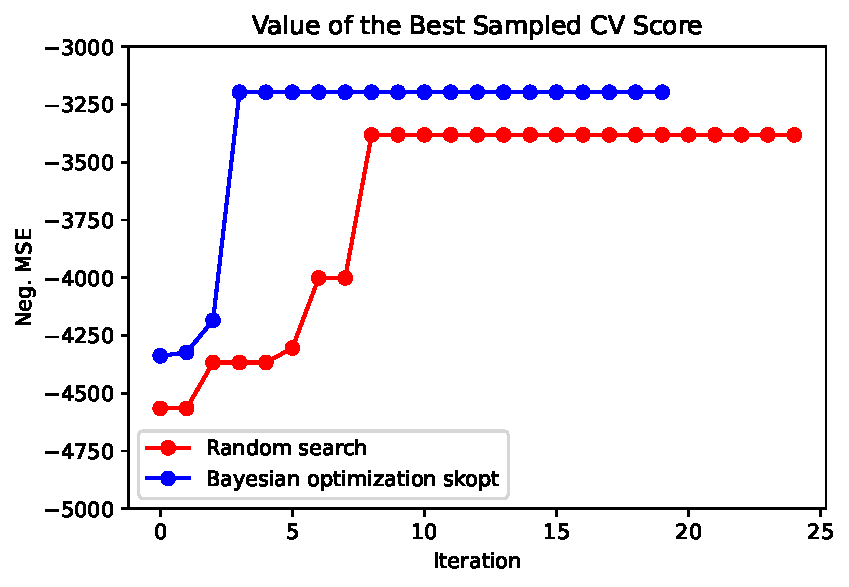
\includegraphics{ProyFinal_OptBayesiana_2024_files/figure-pdf/cell-16-output-1.pdf}

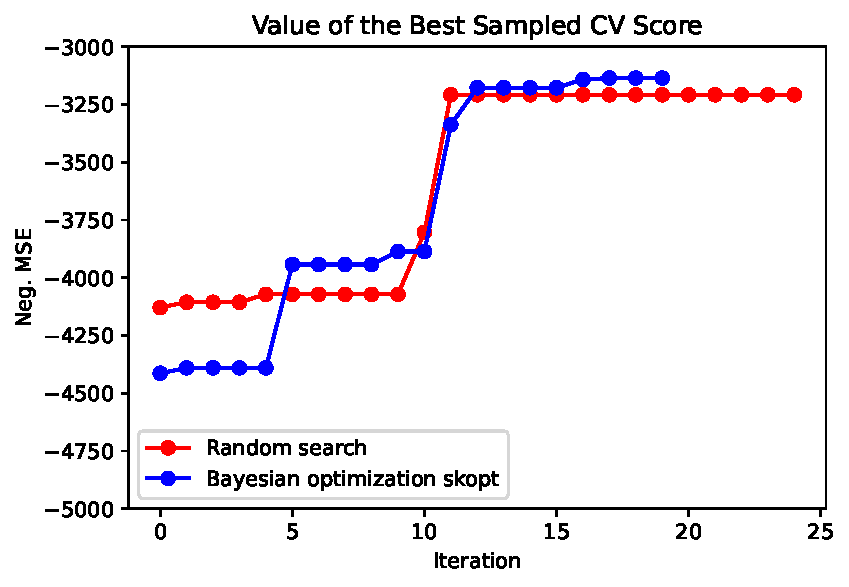
\includegraphics{ProyFinal_OptBayesiana_2024_files/figure-pdf/cell-17-output-1.pdf}

\begin{longtable}[]{@{}lll@{}}
\toprule\noalign{}
& Method & Neg. MSE \\
\midrule\noalign{}
\endhead
\bottomrule\noalign{}
\endlastfoot
0 & Baseline & 4000.175 \\
1 & Random Search & -3381.370 \\
2 & Bayesian Optimization (skopt) & -3196.807 \\
3 & Bayesian Optimization (GPyOpt) & -3145.947 \\
\end{longtable}

\subsubsection{California Housing
Prices}\label{california-housing-prices}

En este ejemplo, aplicaremos la optimización bayesiana a un problema de
regresión de precios de vivienda en California. El conjunto de datos se
puede descargar de
\href{https://www.kaggle.com/camnugent/california-housing-prices}{Kaggle}
y contiene información sobre la población, los ingresos medios, los
precios de las viviendas, etc. El objetivo, es predecir los precios de
las viviendas en función de las características proporcionadas.

\paragraph{Ajuste de hiperparámetros con búsqueda
aleatoria}\label{ajuste-de-hiperparuxe1metros-con-buxfasqueda-aleatoria-1}

Para el ajuste de hiperparámetros con búsqueda aleatoria, utilizamos
\texttt{RandomSearchCV} de scikit-learn y calculamos una puntuación de
validación cruzada para cada punto seleccionado aleatoriamente en el
espacio de hiperparámetros. El modelo utilizado fue
\texttt{GradientBoostingRegressor} de scikit-learn.

\paragraph{Ajuste de hiperparámetros con optimización
bayesiana}\label{ajuste-de-hiperparuxe1metros-con-optimizaciuxf3n-bayesiana-1}

Para ajustar los hiperparámetros con optimización bayesiana,
implementamos una función objetivo \texttt{cv\_score} que toma los
hiperparámetros como entrada y devuelve una puntuación de validación
cruzada. El modelo, empleado fue \texttt{GradientBoostingRegressor} de
scikit-learn.

\begin{verbatim}
Baseline neg. MSE = 0.45815
Random search neg. MSE = 0.44542
Bayesian optimization GPyOpt neg. MSE = 0.38734
\end{verbatim}

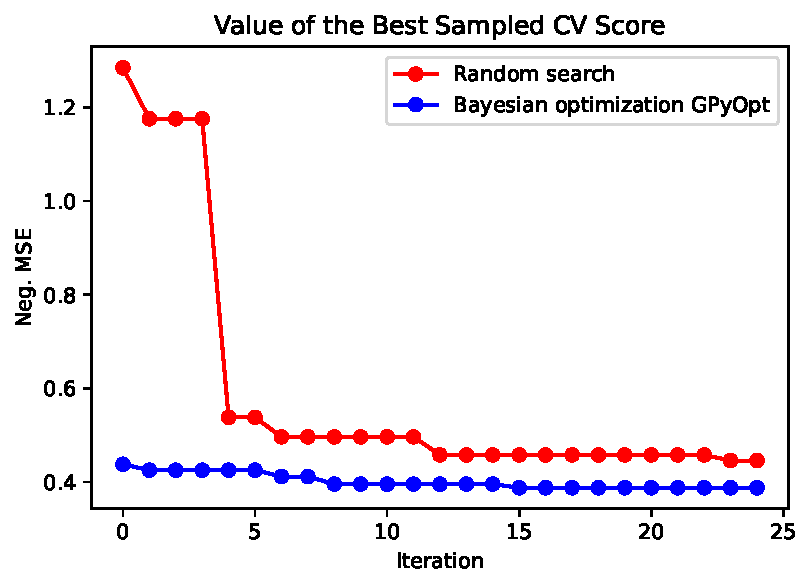
\includegraphics{ProyFinal_OptBayesiana_2024_files/figure-pdf/cell-23-output-1.pdf}

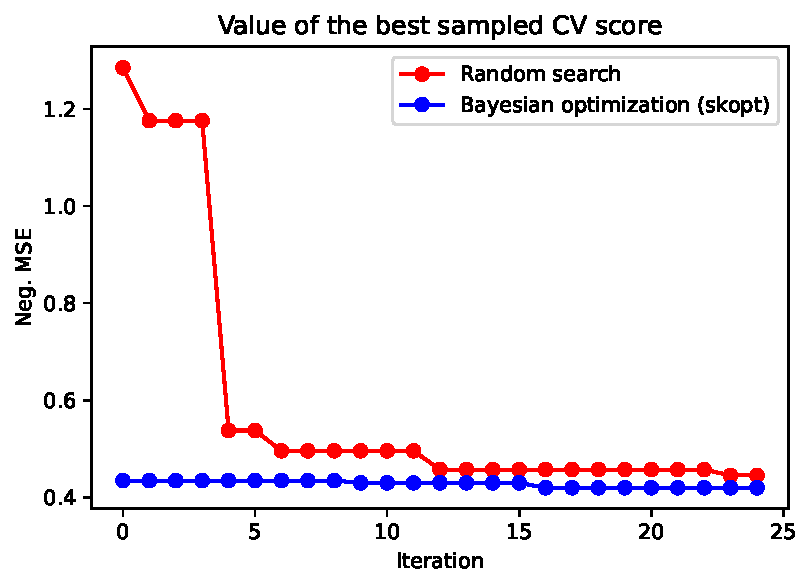
\includegraphics{ProyFinal_OptBayesiana_2024_files/figure-pdf/cell-24-output-1.pdf}

\begin{longtable}[]{@{}lll@{}}
\toprule\noalign{}
& Method & Neg. MSE \\
\midrule\noalign{}
\endhead
\bottomrule\noalign{}
\endlastfoot
0 & Baseline & 0.45815 \\
1 & Random Search & 0.44542 \\
2 & Bayesian Optimization (skopt) & 0.41997 \\
3 & Bayesian Optimization (GPyOpt) & 0.38734 \\
\end{longtable}

\section{Fuentes}\label{fuentes}

\begin{itemize}
\tightlist
\item
  {[}\#{]} Bradley Efron, Trevor Hastie, Iain Johnstone and Robert
  Tibshirani (2004) ``Least Angle Regression,'' Annals of Statistics
  (with discussion), 407-499.
  (https://web.stanford.edu/\textasciitilde hastie/Papers/LARS/LeastAngle\_2002.pdf)
\end{itemize}




\end{document}
